\documentclass[bachelor,euler,twoside,openright]{ustcthesis}
% 默认twoside 双面打印
% 将master修改为bachelor, doctor or master
% 要使用adobe字体,添加adobefonts选项
% 使用euler数学字体,如不愿使用,去掉euler
% 使用外文写作,请添加notchinese

% 设置图形文件的搜索路径
\graphicspath{{figures/}}

%仅用于本示例文档中显示特殊字符串
\usepackage{xltxtra}

%%%%%%%%%%%%%%%%%%%%%%%%%%%%%%
%% 封面部分
%%%%%%%%%%%%%%%%%%%%%%%%%%%%%%

  % 中文封面内容
  \title{基于NDN网络的时间标签多层控制器同步算法}%一般情况下扉页和书脊共用一个标题文本,可以不用定义\spinetitle。特殊情况见下。
  \spinetitle{\small{基于NDN网络的时间标签多层控制器同步算法}}
  %特殊情况1:本例中\title命令里含有换行控制字符,这会导致制作书脊的时候出现错误,
  %  例如如果你注释掉\spinetitle{...}这一行就会报错。
  %  这时需要定义一个不含换行等命令的\spinetitle,这并不表示\spinetitle里不能有任何命令——只能使用有限的命令。
  %特殊情况2:本例中标题过长,所以需要缩小书脊标题的字号。
  %特殊情况3:本例中中英文混排,由于tex竖排的原理限制,中英文基线不重合,所以需要人工调整英文的基线。具体调整量根据不同字体有所不同。
  \author{李\ 合\ 璧}
  \depart{自动化系}%系别,硕博请用系代号,本科请用全称如
  \major{自动化}%专业,硕博请用全称,本科不需要
  \studentid{PB10210014}
  \advisor{谭小彬\ 副教授}
  \submitdate{二〇一四年六月}

  % 英文封面内容
  \entitle{Distributed Random Servers With Timed Labels for Synchronization over Named Data Network}
  \enauthor{Hebi Li}
  \enmajor{Automation}
\endepart{Automation}
  \enadvisor{Prof. Xiaobin Tan}
  \ensubmitdate{June, 2014}

\begin{document}

  \maketitle

%特别注意,以下述顺序为准,在对应部分添加文档部件,切勿颠倒顺序:
%本科论文的文档部件顺序是:
%    frontmatter:致谢、目录、中文摘要、英文摘要、
%    mainmatter: 正文章节
%    backmatter: 参考文献或资料注释、附录
%硕博论文的文档部件顺序是:
%    frontmatter:中文摘要、英文摘要、目录、符号说明
%    mainmatter: 正文章节
%    backmatter: 参考文献、附录、致谢、发表论文
%%%%%%%%%%%%%%%%%%%%%%%%%%%%%%
%% 前言部分
%%%%%%%%%%%%%%%%%%%%%%%%%%%%%%
\frontmatter
\makeatletter
\ifustc@bachelor
	%%%%%%%%%%%%%%%%%
	%本科论文修改这里
	%%%%%%%%%%%%%%%%%
	% 致谢
	
\begin{thanks}


在中国科技大学完成本科学业的四年里,我所从事的学习和研究工作,都是在导师以及系里其他老师和同学的指导和帮助下进行的。
在完成论文之际,请容许我对他们表达诚挚的谢意。

首先感谢导师谭小彬副教授这一年的指导和教诲,是他们把我带到了未来网络的研究领域。
在完成毕业设计的过程中,每一次与谭老师的讨论都让我的思路更清晰,他的一针见血的提问不断纠正我前进的方向.
谭老师严谨的研究态度及忘我的工作精神,认真细致的治学态度及宽广的胸怀,都将使我受益终身。

感谢班主任陈金雯老师多年的关怀。
感谢朱明,郑烇等老师,他们的指导给我本科阶段的研究工作打下了基础。

感谢周子健、周自飞、武帆等师兄师姐们的指点和照顾;
感谢肖琪、赵志凡、陈杨斌等几位同班同学,与你们的讨论使我受益良多;
我们在1316实验室共同学习共同生活,一起走过了这段愉快而难忘的岁月。

感谢科大,感谢一路走过来的兄弟姐妹们,在最宝贵年华里,是你们伴随着我的成长。

最后,感谢我家人一贯的鼓励和支持,你们是我追求学业的坚强后盾。

\vskip 18pt

\begin{flushright}

~~~~李合璧~~~~

\today

\end{flushright}

\end{thanks}


	%目录部分
	%目录
	\tableofcontents
	%默认表格、插图、算法索引名称分别为“表格索引”、“插图索引”和“算法索引”
	%如果需要自行修改lot,lof,loa的名称,请定义
	%\ustclotname{...}
	%\ustclofname{...}
	%\ustcloaname{...}

	% % 表格索引
	% \ustclot
	% % 插图索引
	% \ustclof
	% %算法索引
	% %如果需要使用算法环境并列出算法索引,请加入补充宏包。
	% \ustcloa

	% 摘要
	
\begin{cnabstract}
作为新一代因特网架构,NDN网络提供了很多新的特性,使传统的IP网络的诸多缺点的得以克服。
群聊软件,如QQ群聊,视频会议等,需要保证群体中的每个人都能收到其他所有人所发布的消息。
传统因特网需要有一台中央服务器,收集每个人的消息,并推送给其他人。
这种结构存在严重的overhead,较长的实验,并且鲁棒性不强。
本研究课题充分利用NDN网络分布式的特点,并利用缓存和interest聚合实现数据同步的算法。

在这篇论文中,我们提出了基于NDN网络的解决即时多人聊天应用的新的算法,TreeSync。
TreeSync充分利用了传统中央服务器式模型和NDN的有效的分布式特性。

首先,多层控制节点可以提供强大的控制能力,来处理复杂的情形。
其次,该设计的本质的分布式特征让它能够有效率的获取消息,并且具有鲁棒性和移动性支持,享有极小的overhead。
另外,树形结构的层级设计也为扩展性提供了保证。当节点增多时,复杂度是指数下降的。

我们在ndnSIM上实现了TreeSync,并且评估了其性能。消息能够正确而快速的在群体中相互同步。
在拥有较快同步时延的同时,overhead相对于其他算法有显著的降低。

\keywords{NDN,消息同步}
\end{cnabstract}


\begin{enabstract}

Key problem of multi-user real-time communication applications,
such as group chat and video conference,
is how to synchronize messages among all participants.
Traditional IP-based way depends on central server, resulting in unbalanced link burden and robust problem.
A recent solution on NDN, ChronoSync, has several crucial limitations.
In this paper, we propose a new distributed algorithm based on Named Data Network to address this problem.
In our design, the system generates a tree topology according to the real one.
Every node takes responsibility to synchronize its children and bubble messages up to its parent.
On receiving control messages from upper node,
participants send request to the real message directly, taking advantage of NDN's consumer-driven design.
This method synthesizes the powerful control ability of servers and NDN's distributed features.
We implemented TreeSync on ndnSIM and compared it with ChronoSync.
It proved small overhead and fast synchronization.

In this paper, we proposed TreeSync, a new algorithm to handle the synchronization problem in multi-user applications.
TreeSync takes advantages of both traditional server-based model and NDN's neat and efficient distributed features.
First of all, Multi-level controllers can provide enough control ability to handle complex conditions;
Secondly, The essential distributed features allow it to fetch data efficiently and robustly with little overhead;
Besides, The hierarchy structure makes the algorithm scalable.
We have implemented TreeSync over ndnSIM and evaluated the performance.
Message is correctly and fast synchronized in a distributed way.
With a reasonable delay of sync control message transmission,
the overhead is much lower due to powerful control ability.


\enkeywords{NDN, Message Synchronization}
\end{enabstract}
%此文件中含有中英文摘要
\else
	%%%%%%%%%%%%%%%%%
	%硕博论文修改这里
	%%%%%%%%%%%%%%%%%
	% 摘要
	
\begin{cnabstract}
作为新一代因特网架构,NDN网络提供了很多新的特性,使传统的IP网络的诸多缺点的得以克服。
群聊软件,如QQ群聊,视频会议等,需要保证群体中的每个人都能收到其他所有人所发布的消息。
传统因特网需要有一台中央服务器,收集每个人的消息,并推送给其他人。
这种结构存在严重的overhead,较长的实验,并且鲁棒性不强。
本研究课题充分利用NDN网络分布式的特点,并利用缓存和interest聚合实现数据同步的算法。

在这篇论文中,我们提出了基于NDN网络的解决即时多人聊天应用的新的算法,TreeSync。
TreeSync充分利用了传统中央服务器式模型和NDN的有效的分布式特性。

首先,多层控制节点可以提供强大的控制能力,来处理复杂的情形。
其次,该设计的本质的分布式特征让它能够有效率的获取消息,并且具有鲁棒性和移动性支持,享有极小的overhead。
另外,树形结构的层级设计也为扩展性提供了保证。当节点增多时,复杂度是指数下降的。

我们在ndnSIM上实现了TreeSync,并且评估了其性能。消息能够正确而快速的在群体中相互同步。
在拥有较快同步时延的同时,overhead相对于其他算法有显著的降低。

\keywords{NDN,消息同步}
\end{cnabstract}


\begin{enabstract}

Key problem of multi-user real-time communication applications,
such as group chat and video conference,
is how to synchronize messages among all participants.
Traditional IP-based way depends on central server, resulting in unbalanced link burden and robust problem.
A recent solution on NDN, ChronoSync, has several crucial limitations.
In this paper, we propose a new distributed algorithm based on Named Data Network to address this problem.
In our design, the system generates a tree topology according to the real one.
Every node takes responsibility to synchronize its children and bubble messages up to its parent.
On receiving control messages from upper node,
participants send request to the real message directly, taking advantage of NDN's consumer-driven design.
This method synthesizes the powerful control ability of servers and NDN's distributed features.
We implemented TreeSync on ndnSIM and compared it with ChronoSync.
It proved small overhead and fast synchronization.

In this paper, we proposed TreeSync, a new algorithm to handle the synchronization problem in multi-user applications.
TreeSync takes advantages of both traditional server-based model and NDN's neat and efficient distributed features.
First of all, Multi-level controllers can provide enough control ability to handle complex conditions;
Secondly, The essential distributed features allow it to fetch data efficiently and robustly with little overhead;
Besides, The hierarchy structure makes the algorithm scalable.
We have implemented TreeSync over ndnSIM and evaluated the performance.
Message is correctly and fast synchronized in a distributed way.
With a reasonable delay of sync control message transmission,
the overhead is much lower due to powerful control ability.


\enkeywords{NDN, Message Synchronization}
\end{enabstract}
%此文件中含有中英文摘要
	% 目录
	\tableofcontents
	%默认表格、插图、算法索引名称分别为“表格索引”、“插图索引”和“算法索引”
	%如果需要自行修改lot,lof,loa的名称,请定义
	%\ustclotname{...}
	%\ustclofname{...}
	%\ustcloaname{...}

	% 表格索引
	\ustclot
	% 插图索引
	\ustclof
	%算法索引
	%如果需要使用算法环境并列出算法索引,请加入补充宏包。
	\ustcloa

	%符号说明,需要加入补充包
	\begin{denotation}

\item[HPC] 高性能计算 (High Performance Computing)
\item[cluster] 集群
\item[Itanium] 安腾
\item[SMP] 对称多处理
\item[API] 应用程序编程接口
\item[PI]	聚酰亚胺
\item[MPI]	聚酰亚胺模型化合物,N-苯基邻苯酰亚胺
\item[PBI]	聚苯并咪唑
\item[MPBI]	聚苯并咪唑模型化合物,N-苯基苯并咪唑
\item[PY]	聚吡咙
\item[PMDA-BDA]	均苯四酸二酐与联苯四胺合成的聚吡咙薄膜
\item[$\Delta G$]  	活化自由能~(Activation Free Energy)
\item [$\chi$] 传输系数~(Transmission Coefficient)
\item[$E$] 能量
\item[$m$] 质量
\item[$c$] 光速
\item[$P$] 概率
\item[$T$] 时间
\item[$v$] 速度
\end{denotation}
%不是必需的,如果不想列出请注释掉
\fi
\makeatother

%%%%%%%%%%%%%%%%%%%%%%%%%%%%%%
%% 正文部分
%%%%%%%%%%%%%%%%%%%%%%%%%%%%%%
\mainmatter

  % \include{chapter/chap-intro}
  % \include{chapter/chap-guide}
  % \include{chapter/chap-example}
  %自行添加
  %\include{chapter/...}
  
\chapter{绪论}

\section{数据命名网络}

数据命名网络,Named Data Network\cite{zhang2010named},简称NDN,是未来因特网架构的一部分。
该项目项目旨在开发一个新的互联网架构,可以对互联网目前的基于主机的,点至点的通信体系结构的和地址的弱点进行优化。
该项目研究并加以解决以下问题,以验证NDN作为未来互联网体系结构的技术挑战:
路由的可扩展性,快进,信任模型,网络安全,内容保护和隐私,以及基本的传播理论。
该NDN项目已于2010年9月资助的美国国家科学基金会NSF下的未来互联网体系结构项目的四个项目之一。
不同于现有的IP网络,NDN中不使用端到端的解决方案。


\begin{figure}
\centering
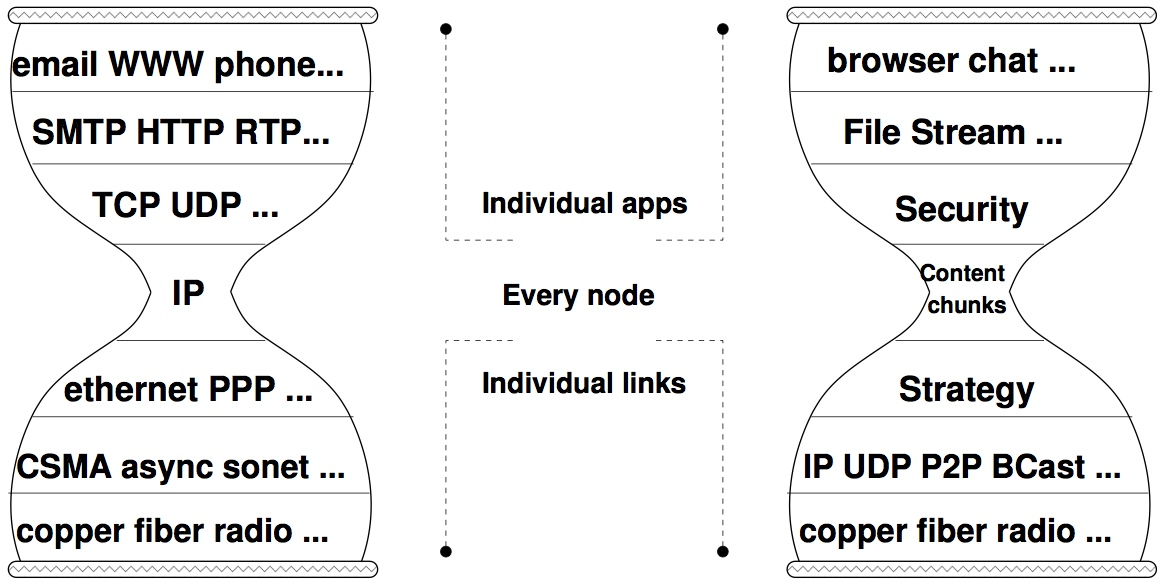
\includegraphics[width=4.5in]{png/ndn_and_ip.jpg}
\caption{NDN和IP的架构比较}
\label{fig:hour_glass}
\end{figure}

\begin{figure}[]
\centering
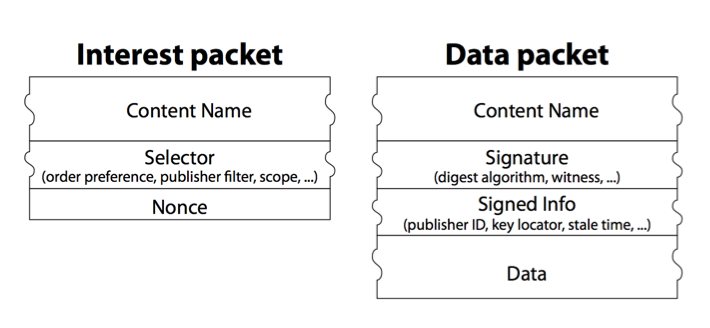
\includegraphics[width=4.5in]{png/ndn_packet.png}
\caption{NDN中得Interest和Data数据包}
\label{fig:interest_data}
\end{figure}

如图\ref{fig:hour_glass}所示,不同于IP的`hour glass'架构,
在NDN通信接收端,数据数据是由消费者驱动的。
在NDN中,存在两种包格式:兴趣包和数据包,如图\ref{fig:interest_data}.
接收数据时,消费者发出一个兴趣分组,它带有用于识别所需要的数据的名称。
例如,消费者可以请求`/ustc/video/a.mpg'。
路由器记得该请求进入的端口,然后在其转发的转发兴趣报列表(FIB )中查找名称。
它是一个基于名字的路由协议。
当兴趣包达到具有所请求的数据的节点时,一个数据包被发送回,
它带有两个名称和内容数据,并带有生产者的签名。
此数据包沿着兴趣分组的反向的路径,回到消费者。
需要注意的是,无论是兴趣包还是数据包,都不携带任何主机或接口地址(如IP地址)。
兴趣包路由到数据是基于兴趣包所包含的报文的名字,数据包产生者根据由兴趣包在每个路由器跳状态信息原路返回。
NDN路由器保持兴趣包和数据一段时间,作为缓存。

\begin{figure}
\centering
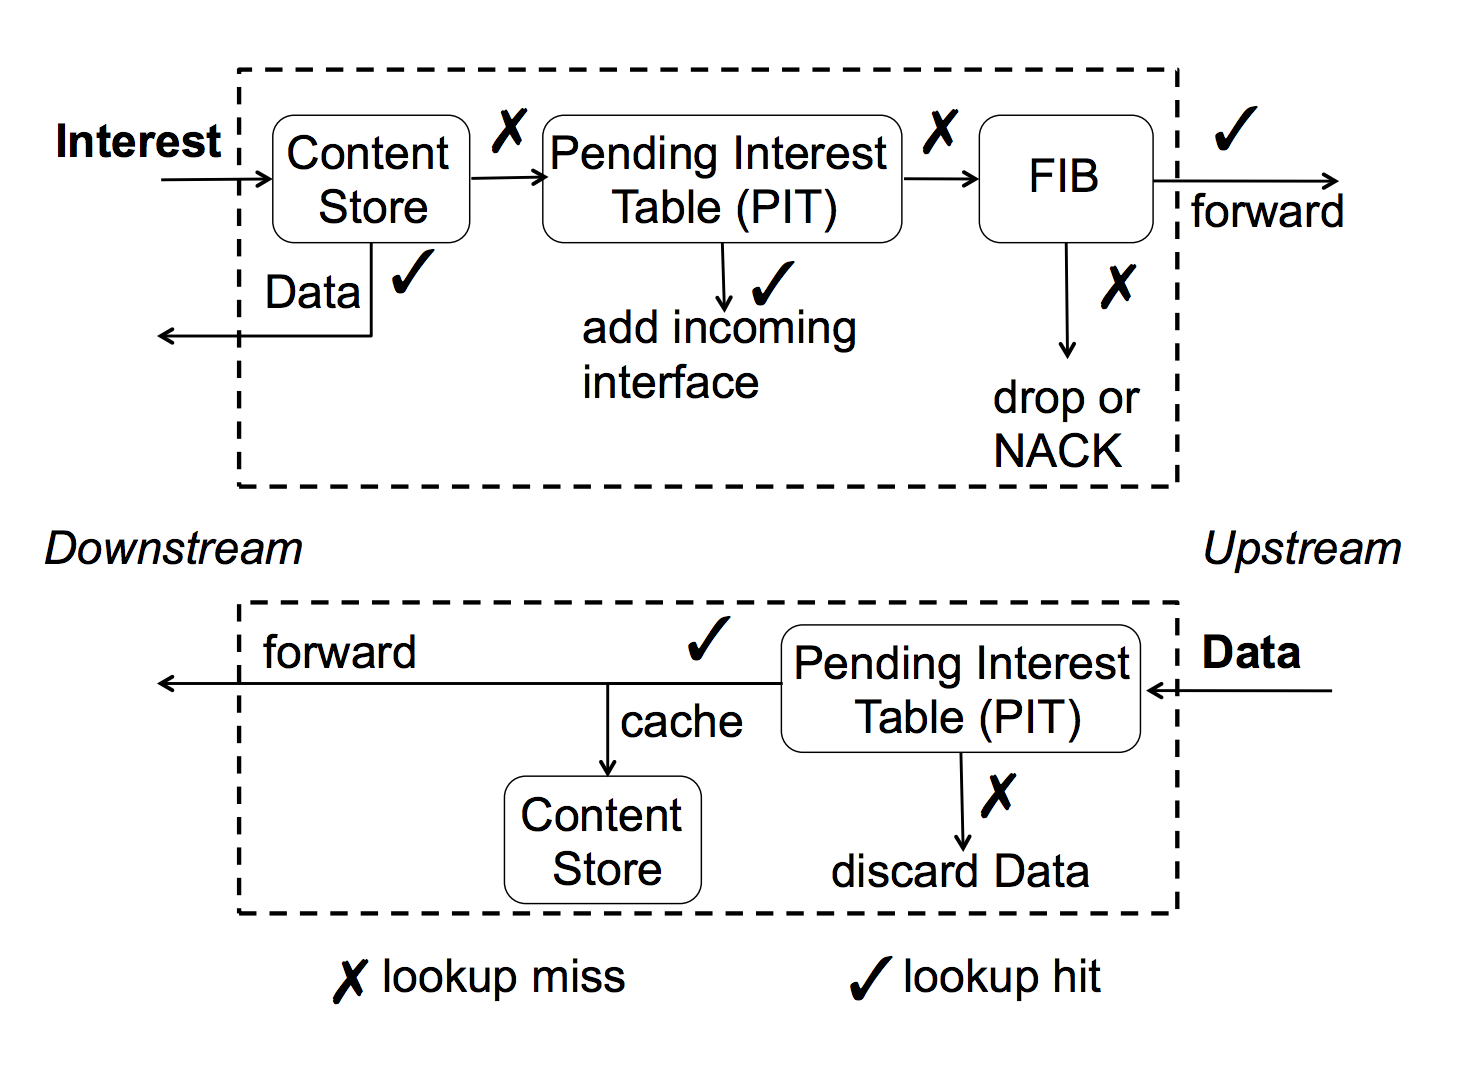
\includegraphics[width=4.5in]{png/interest_data_process.png}
\caption{NDN中处理Interest和Data数据包的流程}
\label{fig:ndn_process}
\end{figure}

在NDN中处理兴趣包时,如图\ref{fig:ndn_process},先查找自己的CS.
如果找到,那么直接返回这个数据,不会将Interest向下一跳传递.
如果没有找到,他会查看自己的PIT表,如果存在,那么在PIT表中添加此端口后丢弃.
这就保证了不会有相同的Interest在同一个链路中传递.
如果PIT中也没有,路由器就会在FIB中查找该名称,以确定向那个端口转发此兴趣包.
如果FIB中也没有,那么返回错误信息.
图\ref{fig:forwarding}描述了这个转发兴趣包的过程.

当多个相同兴趣包所请求的为同一个数据,那么只有第一个对数据源的兴趣包会向上游发送。
该路由器然后将这个转发信息存储在转发兴趣包表( PIT )中 ,
其中每个条目包含兴趣包名和一组从接口,这些接口都是发送该兴趣包来的接口。
当数据包到达时,路由器就会找到与之对应的PIT项和数据转发到所有列出的接口PIT的条目。
路由器然后删除相应的PIT表项,并将其缓存在自己的本地缓存中。
这使用路由器的缓冲存储器,并采用高速缓存替换策略。
数据有请求它的兴趣包的精确相同的路径,但是传输方向相反。
PIT和FIB的结构见图\ref{fig:pit_fib}.

\begin{figure}
\centering
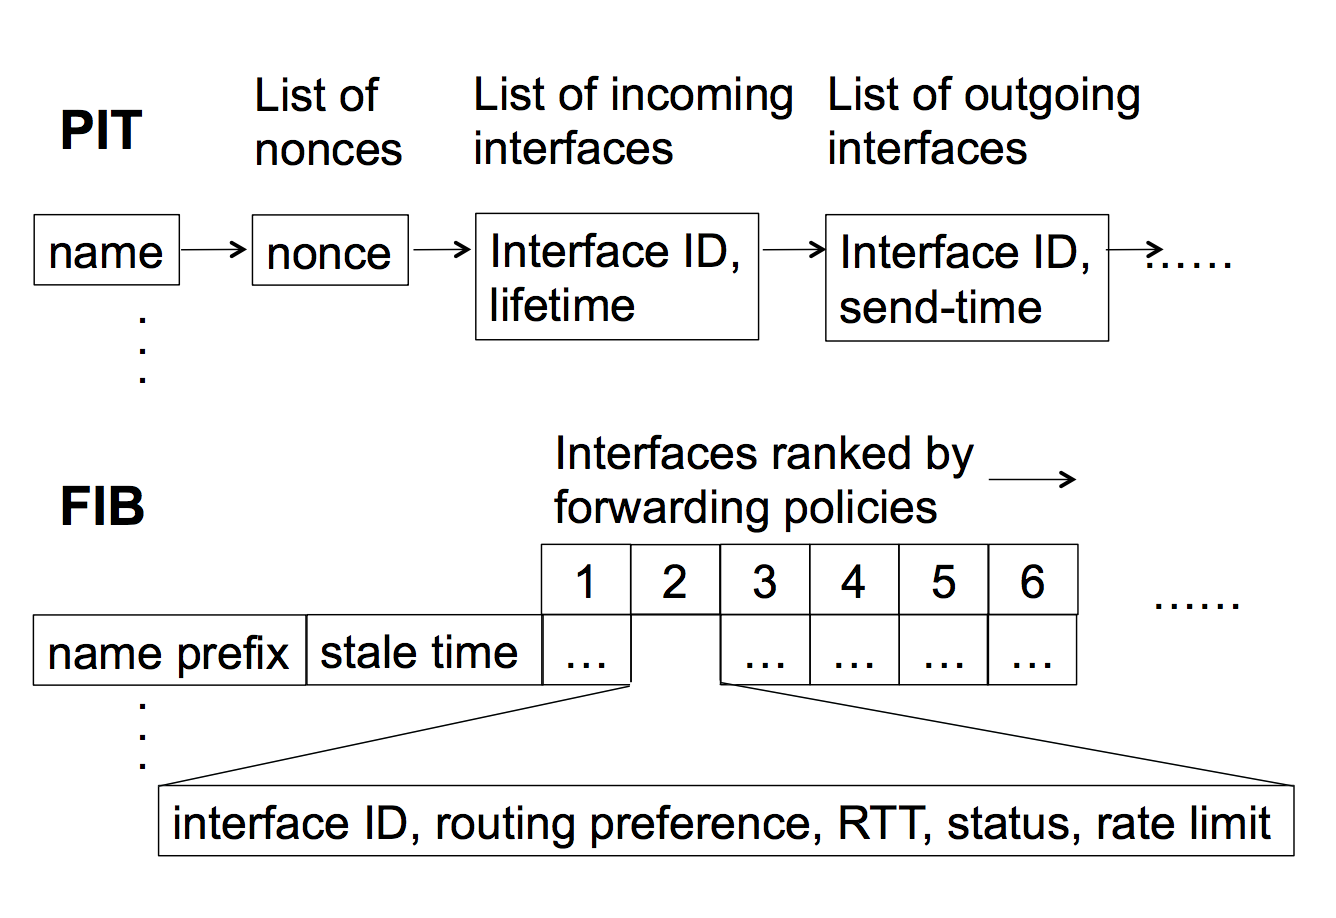
\includegraphics[width=4.5in]{png/pit_fib.png}
\caption{PIT和FIB的结构}
\label{fig:pit_fib}
\end{figure}

\begin{figure}
\centering
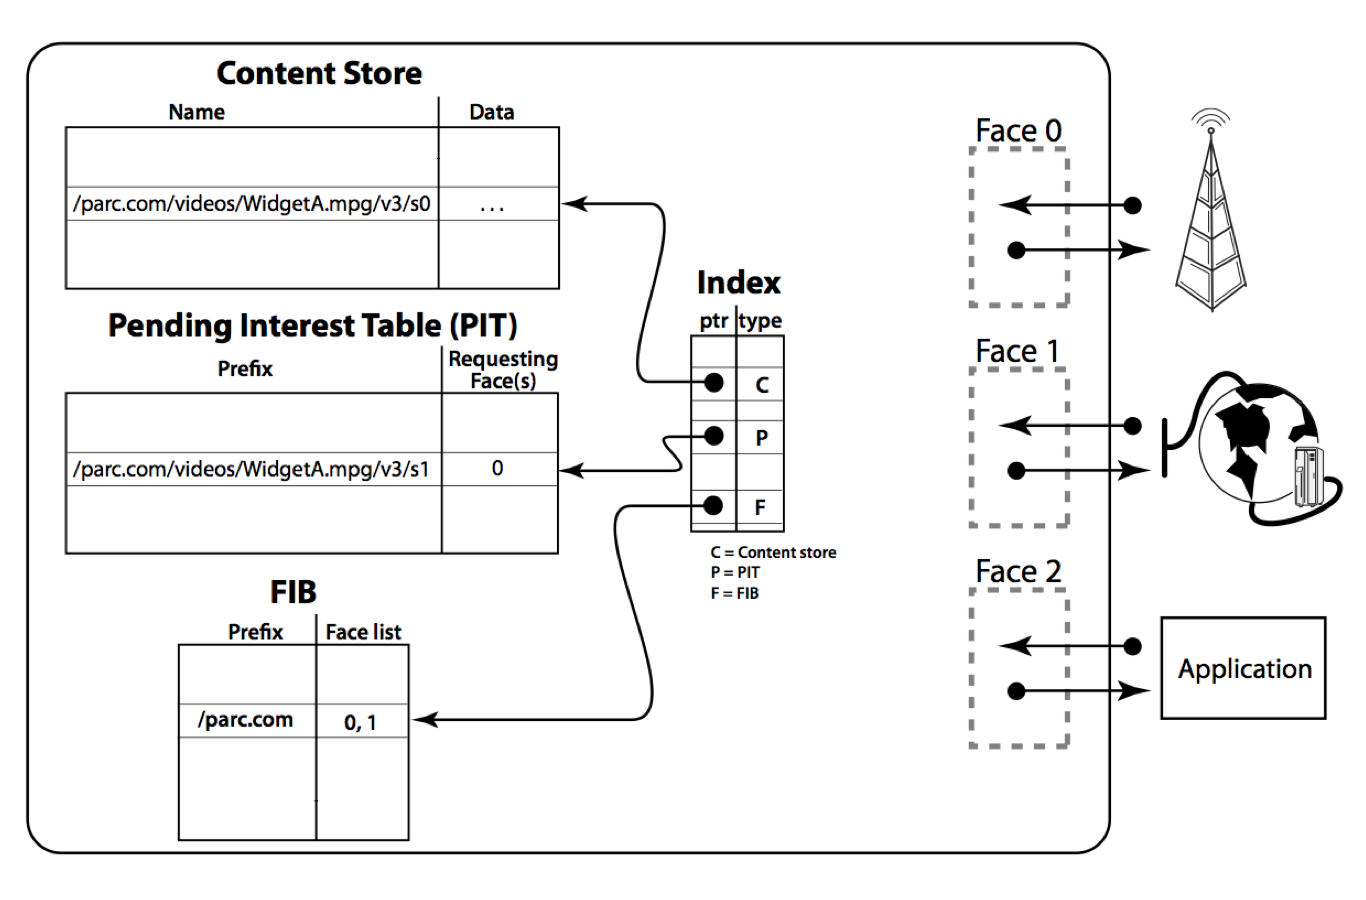
\includegraphics[width=4.5in]{png/forwarding.png}
\caption{一个NDN节点对数据包的转发过程}
\label{fig:forwarding}
\end{figure}


一个数据满足一个兴趣包,在每个跃点,实现逐跳流量平衡。
一个NDN数据包与其是来自何处,或在有可能被转发到的位置是独立的,
因此,路由器可以缓存它来满足未来的潜在需求。
这使NDN自动支持各种功能,而无需额外的基础设施,
包括内容分发(许多用户要求在不同的时间相同的数据),
多播(许多用户请求相同的数据在同一时间),
流动性(用户请求来自不同位置的数据),
并延迟容忍网络(用户有间歇连接)。
例如,考虑一个消费者在移动的车辆中观看流媒体视频。
消费者可以请求一些数据,但然后移动到一个新的本地网络。
虽然数据将在到达旧的位置和被丢弃,但是沿着路径会被缓存。
当消费者重发兴趣包,它可能会从附近的一个缓存中提取数据,使得中断最小。
数据缓存接近消费者提高网络传输性能,并减少对特定数据源的依赖。
这样就能有效避免由于故障或攻击可能导致的失败。

\section{即时多人聊天应用的数据同步问题}

即时多人聊天应用,例如qq,msn等热门应用,
所提供的关键功能是让群体中的每一个人都能向群体中发送消息,接受消息。
不同于两人聊天,多人聊天就涉及到如何让所有人都能收到其他人所发送的消息。
现阶段,此类应用都是运行在现有网络,即IP网络上的。这为其带来了不可避免的弊端。

IP网络被设计成点对点的通信,即通信过程中,整个网络层所知道的是通信源点和目标节点的IP地址。
路由器根据IP地址解析出下一跳的路径,并传递数据包。

在IP网络上,这些应用的同步算法是要有中央服务器的。每个人都和中央服务器建立连接。
中央服务器负责收集每个人的发送的消息,并将这些消息转发给其余所有人。
当一个参与者发送了一条文本信息,此信息会先经过路由到达中央服务器。
中央服务器维护了一个包含所有参与者的列表,
它收到消息后,经过计算处理,然后将此消息转发给需要它的人,以完成功能。

虽然这种办法可行,而且实际上在IP网络上也只能这样运行。
但是这种方法带来了严重的性能问题。

\begin{enumerate}
\item 存在大量的overhead

由于IP是点对点通信,这意味着中央服务器想要将一个消息传递给一个聊天室里的所有成员时,
不得不建立与所有人的TCP连接,并向每一个连接发送一份消息的副本。
如果有两个聊天用户在拓扑上非常近(例如他们连在同一个路由器上,而服务器可能在十跳之外。
这种情况下,需要两个相同的数据包,在这十个路由器上经过,而事实上只需要一个。
在群聊的环境中,用户量更大,更密集,从而造成更加大得多的overhead。
\item 鲁棒性不强

由于所有通信的实现都需要中央服务器的调节,这造成了单点故障。
如果服务器宕机了,或者被不法分子攻击,整个网络中的所有成员均不能正常通讯。
系统也无法自我修复,必须等到服务器维修好后才能重新上线服务。
\end{enumerate}


IP的点对点的通讯模型导致了这些性能瓶颈,
而Named Data Network作为最近发展的一个新的网络架构,为解决这个问题提供了机会。
NDN的优于IP网络模型的根本点在于它不是点对点的模型。
NDN中,所有的资源使用一个独一无二的名字来索引,每个名字对应了一个资源。
资源获取是消费者主导的,也就是说,客户端想要访问一个资源时,
他以此资源的名字发送Interest数据包,并等待接受返回的数据。
由于资源是以名字来定义的,所有请求同一个资源的用户所发送的请求都是一样的:资源的独一无二的名字,
那么NDN中的路由器就会检测到相同的兴趣包,而不会将这个重复的兴趣包向下一跳传递。
当有内容返回时,NDN路由会将这个数据包向所有的端口转发,从而实现多路转发。
除此之外,NDN路由还涉及了缓存机制,当有内容数据包返回时,它会将这个包缓存在自己的内存中。
如果之后有用户请求相同的资源,NDN路由就会发现这个资源已经在自己的缓存中了,于是便可以直接返回给客户端。
这显著的减少了overhead,而且加快了数据包响应时间。

基于NDN的这些特性,它可以为即时多人聊天应用提供很好的架构基础,为解决这个性能瓶颈提供了新的机会。
利用这些特性,以上的问题可以得到较好的解决。
由于NDN的资源是有独特名字的,聊天室里的每一个人想要得到最新消息时,发送的兴趣包是相同的。
NDN路由会过滤掉所有重复的兴趣包,而往下一个路由只发送一份。
当数据返回时,内容包也会只有一份传递回来,并且由路由向各个端口分发数据包。
这样就实现了比传统IP方式小得多的overhead。
另一个方面,由于NDN不关心端点的IP,所有流量都是由Interest包的名字决定的,
因此可以将算法设计成分布式的,当有些节点出现故障,系统仍然可以继续工作,并且可以自我修复。

最近NDN研究人员提出了一种基于此的解决方案,ChronoSync\cite{zhu2013let}。
这个方案是一个完全的分布式的算法,每一个用户都要定期向整个系统广播一个代表他自己当前状态的Interest。
任何人都可以回复这条Interest,只要他认识这个状态,而且他自己的状态更新。
在系统稳定时,每个人都会保留着其他人的Interest,
一旦自己有消息要发送,便立即响应这些Interest,从而将消息发布给团体里的所有人。

ChronoSync为此问题提供了很好的尝试和解决方案,也证明了比IP为基础的算法有明显的优势。
然而,这个算法仍有严重的不足。最大的问题在于,它是一个完全分布的算法,系统没有能力处理特殊情况。
例如,当有两个成员同时发布消息,他们都会响应所保留的别人发来的Interest。
然而,在NDN中,一个Interest只能带回一个数据包,这就必然导致有一个人的消息无法到达。
这样,系统就被分为两个不同阵营,各自有着不同的消息状态,互相无法识别。
更加糟糕的是,当系统里有很多人,出现这种情况的几率将会非常普遍,系统甚至会被分成若干个不同的阵营。
另外,ChronoSync的设计就决定了它无法扩展。每个人需要向全网广播兴趣包,来获取新的消息。
这样这个系统就只能在有限的小范围内使用,如果想在大范围内使用,就必须有分层机制,让复杂度指数递减。

在这种情况下,我们提出了TreeSync来解决此问题。我们的设计目标有以下几点:

\begin{enumerate}
  \item 必须是分布式的。这样才能是系统更健壮,鲁棒性更强。
  \item 有能力处理特殊情况,包括多个并发的消息。
  \item 要能在大范围内进行扩展。
\end{enumerate}

我主要完成的工作有:

\begin{enumerate}
  \item 设计了TreeSync来解决NDN中即时多人聊天应用的信息同步问题。
  \item 在ndnSIM\cite{afanasyev2012ndnsim}中做了仿真。
  \item 与ChronoSync做对比,证明算法的优越性。
\end{enumerate}

接下来各章将会按照如下方式展开。
在第\ref{chapter:relatedwork}章,将会讨论现有的工作,ChronoSync,以及其不足.
第\ref{chapter:design}章,将会详细讨论算法的设计细节。
第\ref{chapter:simu}章叙述在ndnSIM中的仿真情况,并将结果与ChronoSync作对比。
我们将在第\ref{chapter:conclude}章总结全文,展望未来.

  \chapter{相关工作}
\label{chapter:relatedwork}



这一章,我们主要讨论NDN平台中解决此问题的另一个方案:ChronoSync。
来自加州大学洛杉矶分校的Zhenkai Zhu最近提出了此方案。
这是一个完全分布式和服务器较少的协议。

\section{ChronoSync方案设计和算法}

\begin{figure}
\centering
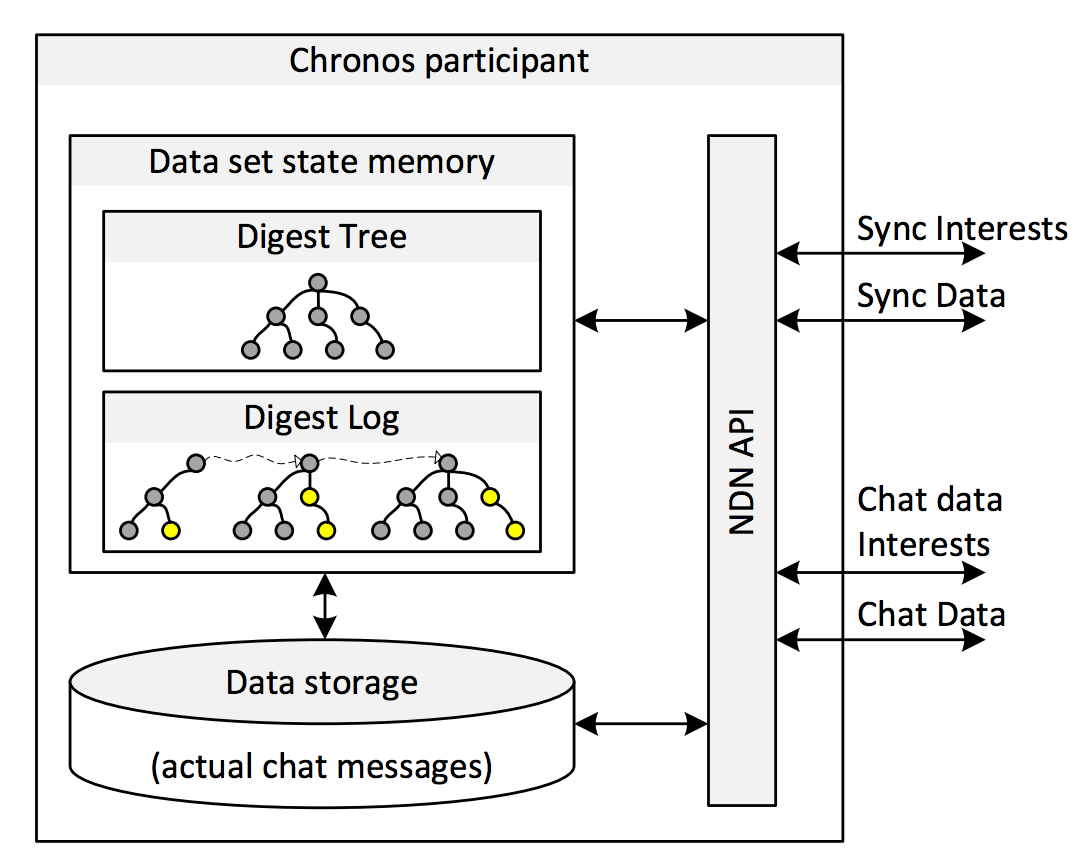
\includegraphics[width=4.5in]{png/digest.png}
\caption{ChronoSync中得摘要树和摘要记录}
\label{fig:digest}
\end{figure}

任何ChronoSync的应用程序的核心是两个相互依存的组件。
同步的数据集的状态的ChronoSync模块,
和响应该数据集的状态的变化的应用逻辑模块。
在ChronoChat ,ChronoSync模块以一个摘要树的形式保持当前用户的所有邮件知识。
在一个摘要日志的形式的数据集的状态变化。
当ChronoSync模块发现聊天室有新的消息,它会通知ChronoChat逻辑模块来获取和存储的消息。

摘要(digest)是ChronoSync中识别一个状态的关键.
如图\ref{fig:digest}所示,每个客户端通过计算自己本地收到的所有人的最新状态,得到一个唯一代表当前状态的摘要.
所有人得摘要集合在一起,组成了根摘要(root digest).
利用这个摘要,每个人就可以相互交流.
当两个人摘要相同时,它们的状态便也是相同的.
当一个人得状态变化时,其摘要也会变化,这时他将前一次状态放入自己本地的摘要记录(digest log)中,用来识别别人的过期的摘要.

为了发现数据集的变化,ChronoSync模块向每个ChronoChat实例发送一个同步的兴趣,
其名称中包含的状态摘要,并将此状态维持在根摘要树。
通常,通过摘要树和摘要日志的帮助,ChronoSync可以直接推断数据集的更改,
以及与包含数据回复到同步感兴趣的变化,这是称为同步数据。

Chronosync仅需要促进有关在数据集中的新数据项的同步,
具体知道了同步信息后做什么是应用程序的工作。
例如,在ChronoChat同步数据带回消息的名字新添加到聊天室,
因而使用者的知识该数据集是带来最新。
然而,用户可 决定是否要取回所有丢失的信息,或只取回最近期的。

\section{ChronoSync的缺点}
\begin{figure}
\centering
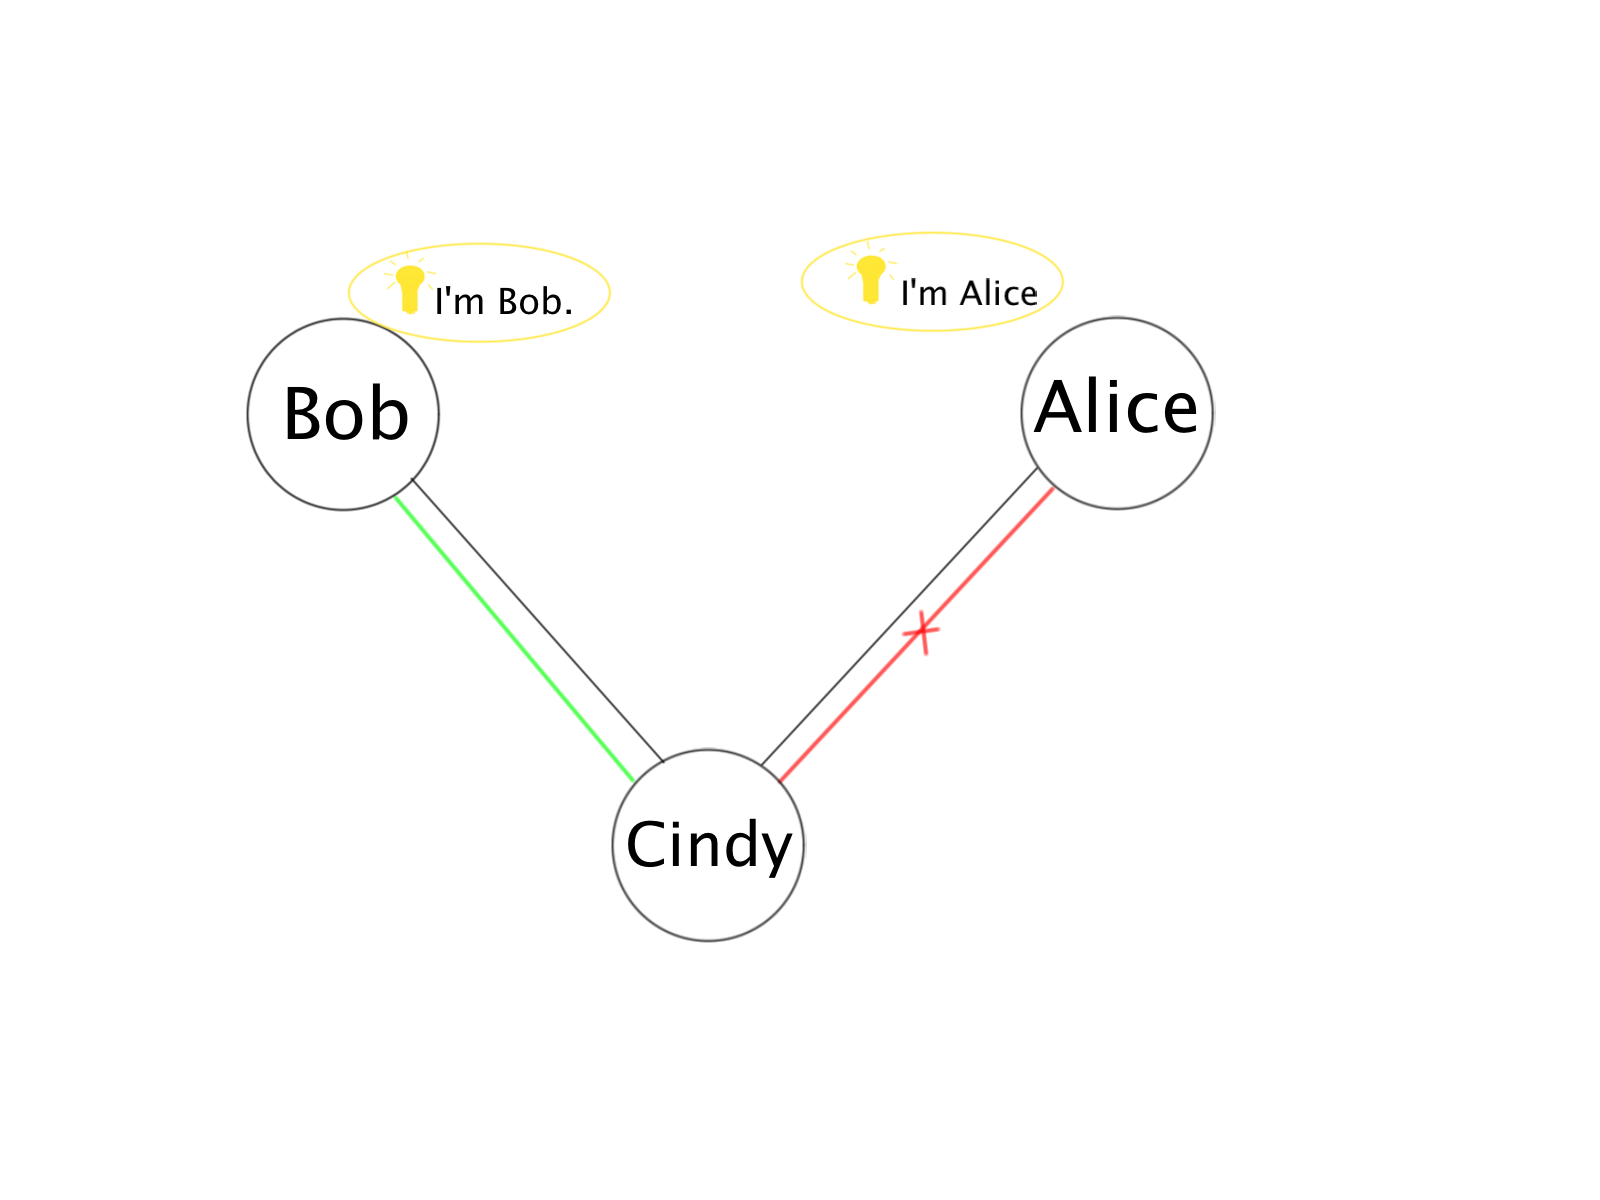
\includegraphics[width=4.5in]{png/simultaneous.png}
\caption{ChronoSync难以解决并发消息产生的问题}
\label{fig:chrono_simultaneous}
\end{figure}

\begin{figure}
\centering
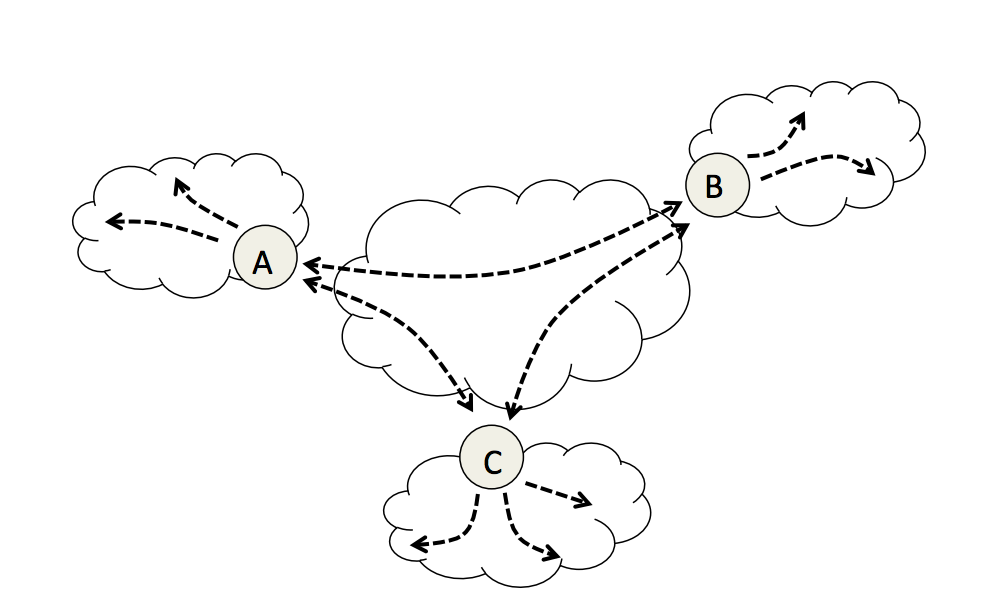
\includegraphics[width=4.5in]{png/chronosync_overlay.png}
\caption{ChronoSync的扩展性问题}
\label{fig:chrono_scalability}
\end{figure}


ChronoSync的主要缺点是控制能力不足,导致在处理并发数据的产生时会有问题。
当这种情况发生时,系统将被分成两个不同的组,并且不能识别来自彼此的摘要。
例如,如图\ref{fig:chrono_simultaneous}所示,
Cindy发出同步的兴趣,要求谁产生一个最新的消息。
如果Alice和Bob说一些在接近的时间,也就是说,
Alice说些什么之前,Bob的话达到Cindy。
在这种方式下,爱丽丝将响应Cindy的同步兴趣,
但它永远不会达到Cindy因为从Cindy同步的兴趣只能取一个数据早在NDN 。
在这个时候,Bob和Cindy都在同一个状态,但Alice是没有的。
本系统被分为两个组,可以不相互识别。

另外一个不足是它不具备可扩展性,只能在较小的范围内使用.
由于没有层级结构,每次发送兴趣包都是要向全网广播,这导致了这种算法不能使用在较大的拓扑结构中.
如图\ref{fig:chrono_scalability}所示,只能在两个相距较远的组之间建立一个覆盖层,并通过这个隧道进行通讯.

  \chapter{TreeSync的设计}
\label{chapter:design}

% 4.1
\section{设计背景}
在本章中,首先分析IP网络和现有NDN解决方案ChronoSync的不足,然后提出我们的设计目标.
\subsection{IP网络的弊端}
IP网络是一个点到点的模型,这意味着每次传输数据时,
路由器并不知道传递的内容是什么,而是按照数据包的源IP和目的IP来转发.
当一个内容由两个用户请求时,该内容必须沿着两个已经建立的连接分别传输到这两个用户,不管他们的距离有多近.
这造成了严重的链路浪费:相同的链路上不停地经过相同的数据包.

在IP网络中,实现分布式的信息交换是很困难的,
因为要想让每一个客户都能将自己产生的数据发送给群体中得所有人,
他必须维护所有其他人的IP地址信息列表,这在互联网中是不现实的.

因此,现有的IP网络中得群聊应用均是建立在中央服务器的基础上,所有人和中央服务器建立连接,将新消息发送给服务器.
服务器将新消息做汇总,并传递给所有参与者.
此方案带来了严重的链路过载,相同的消息沿着每一条TCP连接到达客户端,同一条链路中不停地通过相同的数据包.
另外,这种方案也带来了链路负载的不均衡.靠近中央服务器的链路负载往往非常巨大,而靠近客户端的链路又几乎没有负载.
另一个缺点是该系统的稳定性.由于中央服务器的存在,导致系统存在单点故障隐患.
一旦中央服务器宕机,或者被恶意攻击,整个系统将会崩溃,无法继续完成消息同步的功能.
\subsection{ChronoSync解决方案的不足}
作为分布式消息同步的尝试,ChronoSync提供了NDN上得解决方案.
ChronoSync的设计是完全分布式的,每一个用户向该群体里广播兴趣包,用以拉回新产生的数据.
在NDN中,数据是以名字唯一命名的,因此,
相同的兴趣包不会在同一个链路中传输多次,返回的内容也会沿着相同的路径反向到达客户端.
实验也验证了相对于IP网络传统解决方案的巨大优越性.

然而,ChronoSync存在如下严重的不足.
首先,ChronoSync对于特殊情况的解决没有控制能力.
最主要的是当有消息同时产生时,由于NDN中每一个兴趣包只能拉回一个数据,这时系统就会被分成不能相互认识的两个部分,而无法再相互通讯.
这时候只能通过发送恢复兴趣包来修复此问题.

另一个ChronoSync的设计不足是它无法扩展到大范围的应用.
由于ChronoSync是将兴趣包向全网广播,没有层级结构,这就必然没有可伸缩性,只能在小范围内使用.

\subsection{设计目标}
针对现有IP网络和现有NDN解决方案ChronoSync的不足,我们以如下几点作为我们的设计目标:
\begin{enumerate}
  \item 必须是分布式的。这样才能是系统更健壮,鲁棒性更强。
  \item 有能力处理特殊情况,包括多个并发的消息。
  \item 要能在大范围内进行扩展。
\end{enumerate}

\section{设计思路}
为了得到更强大的控制能力,显然不能放任客户端自己来发送和同步消息.
故而需要有节点来将收到的消息通知进行排序整理,并通知其子节点相关的信息.
这种控制节点的出现会打破分布式的特性,所以这些节点不能是固定的,而是随机产生的.
无论何时,何种控制节点下线或宕机了,系统需要能从这个故障中恢复,即产生另外一个控制节点代替此节点继续工作.
为了具有可伸缩性,系统的拓扑需要是层级形式的,以便系统的复杂度与客户端数目指数递减.
由此,我们设计了具有树形拓扑的随机多层控制器的TreeSync来解决此问题.

\section{设计概述}
在这小节中,我们将要简要讨论整个同步过程。后面的章节将会详细讲述同步的各个部分的细节。

\subsection{树形拓扑}

当有人要加入这个系统,他要做的第一件事就是在系统的拓扑中找到一个位置。
一般的,在最初阶段,每一个人都要找到自己的位置。
每个人会等待一个随机的时间,然后发送“Any Server Interest”请求。
如果他没有收到回复,他将会假设自己是控制器,所以能够去回复别人的“Any Server Interest”请求。
当收到这种回复时,参与者会将他所在节点的父节点设置为收到回复的发起者,并向他索要同步控制信息。
“Any Server Insterest”是和特定层级相关的,这是为多层树结构做准备。

每一个人都要发送心跳包来确定自己的控制节点是否还存在。
一旦检测到其控制节点宕机了,或者由于什么原因下线了,
一个新的控制器会从这个控制器所管辖的客户中选出一个,接替它的位子。
当然,一个新的参与者可以很容易的从他的附近找到一个节点当做自己的控制节点。

\subsection{控制信息}
控制器通过向自己的子节点发送控制信息来主导同步过程。
控制信息并不是真正的数据,而是一种包含什么时间在什么地方有新数据的信息包。
它会告诉接收者,应该在正确的时间到正确的地点拿取数据。
此包中除了包含真正消息的NDN名字,还包含一个标签。
当控制信息顺着拓扑树向下传播时,每一层的控制器都会将自己的名字和他当前的时间加入这个标签。
最终结果是,节点收到的控制信息包中将会包含它上层所有的控制器的名字和时间信息。

\subsection{同步}

当一个节点产生消息,或者更一般的,知道一些新的东西需要向群体中传递,他将会沿着拓扑树向上和向下传递。

向上传递。
当一个节点有新消息要发布,它想他的父节点,也就是他的控制器发送一个带有实际消息名称的Interest。
当控制器收到这个Interest,他将自己的名字和时间添加到这个记录的标签中,然后把它存储在自己本地的日志中。
如果他还有上层节点,它会按照同样的方式向上传递。

向下传递。
为了得到最新的控制信息,每一个用户都会定期向他的控制器发送同步兴趣包,我们称之为“Anything New Interest”。
该包中包含他所知道的最新的标签信息。当一个同步兴趣包超时了,用户会重发此兴趣包。
当控制节点收到该兴趣包后,会和自己的当前知道的最新的标签进行比较。
\begin{enumerate}
  \item 如果标签的时间和他自己的时间是一样的,说明现在他和客户的状态是相同的,此时不需要传递控制信息。
  控制节点会把这个兴趣包保留,以便以后有新的信息时能够迅速响应。
  \item 如果这个标签比他自己的更早,说明该客户的状态已经旧了,需要更新。这时候,他会将用户标签时间点之后的所有新的记录返回给该用户。
  当收到同步兴趣包的返回结果后,客户端会将这个消息记录在自己的日志中,并更新自己的状态。
  这时候他的状态会比他保留的同步兴趣包新,所以会按照相同的方式,继续将此消息向他的子节点传递。
  从而可以达到将控制信息转发给全局的目的。
\end{enumerate}

\subsection{实际消息本体的获取}

当收到控制信息后,每个人都会知道新的消息的NDN名字。
他们直接发送数据请求兴趣包,去向消息产生者索取消息实体。
因为数据的名字在NDN中是唯一的而且稳定不变的,每个参与者的发送的索取相同信息的兴趣包是相同的,
那么这些兴趣包就会被路由聚集,并只发送一份兴趣包的拷贝去下一跳路由。
这就保证了每一个链路中相同的兴趣包只有一个,而不会有重复。当这个兴趣包达到消息产生者后,他会返回消息实体。
此数据包会沿着兴趣包相反的路径传递到所有发送兴趣包的用户,因此overhead非常小。
同时,返回的数据包可以被路由器缓存到本地的内存中,所以当之后有用户请求相同的数据,
他将会直接从临近的路由的缓存里面拿,而不是从消息的产生者那拿。




% 4.2

\section{命名规则}

\begin{table}
\renewcommand{\arraystretch}{1.3}
\caption{使用到的兴趣包的名字}
\label{table:only}
\centering
\begin{tabular}{|c|c|}
\hline
控制节点询问包(ASI) & /broadcast/treesync/anyserver/\emph{level}\\
\hline
新消息通知兴趣包(SNI) & /\emph{server}/treesync/somethingnew/\emph{mylabel}/\emph{dataName}\\
\hline
同步兴趣包(ANI) & /\emph{server}/treesync/anythingnew/\emph{label1:label2:label3}\\
\hline
数据请求兴趣包(DI) & /\emph{publisherName}/treesync/\emph{time}\\
\hline
\end{tabular}
\end{table}

命名是NDN应用程序最重要的部分之一,因为NDN的本质是以名字命名数据。
在这一章,我们简要描述我们在设计中所使用的所有兴趣包的名字。
后面的章节将会分别详细讲述这些兴趣包的用途。

如表\ref{table:only}所示,我们的设计中总共有四中兴趣包的名字。
Anything New Interest 用于产生控制器树形拓扑。
Something New Interest 和 Anything New Interest 用于控制消息的传输。
Data Interest 用来获取真正的消息实体。

名称的第一部分是为了保证路由可以正确的转发它们。
’/broadcast’的兴趣包会被路由到所有相关的端口。
’/serverName’和’/publisher’的兴趣包会被路由到指定的节点。

第二部分’/treesync’是标志当前应用程序的标签。

其他的成分是和具体流程相关的,我们将在后面几章分别讨论。

%4.3

\section{树形拓扑产生}

\begin{figure}
\centering
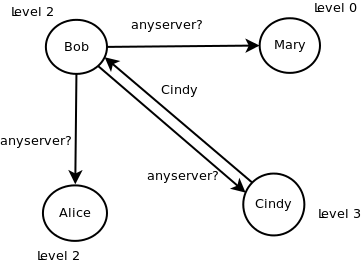
\includegraphics[width=3.5in]{png/server-generation.png}
\caption{控制节点的产生过程}
\label{fig:topo_gen}
\end{figure}

为了产生控制器,我们将使用“Anything New Interest”。
名字的前两部分是为了路由传输和应用处理兴趣包。
第三个部分是兴趣包的类型。
最后一个元素“level”是一个数字,代表了当前这个兴趣包所使用的控制器层级。

在开始阶段,每个人都是独立的没有控制器的。
它们会各自等待一个随机的时间,然后向所有聊天用户广播一个ASI来询问周围有没有控制器。
然后他们会等待一个特定时间Ts。
如果能在Ts过期前收到返回的数据包,它就会将返回此包的用户作为他的父节点,然后发送给他同步兴趣包来索取控制信息。

如果他没有在Ts过期前收到回复,他就会将自己作为一个控制节点,并且准备好回复别的节点的相同的请求。
当区域很大时,在所有一级控制节点之上,会产生更高层的控制节点。
这些节点的生成和之前的算法一样,只是在等待时间上,会和其层级相关,更大的等待时间可以生成更大的区域。
如果在到期之前没有收到回复,控制器就将自己的层级加一。

我们设置一个小的整数,作为最高层级。
只要一个参与者没有上层控制器,而且自己不是最高层控制器,他就会进行这个产生过程。
如果一个节点已经有控制节点,他会向该节点定期发送心跳兴趣包来检测该节点的有效性。
我们将在第七节讨论节点宕机的处理。

注意到控制节点的产生过程和实际拓扑是息息相关的,信息传递的方向当然也是和拓扑相关的。
这就使得经过控制器的延迟不会比直接传递的延迟有显著的增加。
从而保证了传输时延性能。

例如,图\ref{fig:topo_gen},假设当前Bob的层级为2,那么他发送ASI给周围时,
由于Mary和Alice的层级并不大于2,所以都不会回复这个兴趣包.
当兴趣包到达Cindy,由于Cindy的层级为3,可以回复此兴趣包,故Cindy满足此兴趣包.
当Bob收到这个返回的数据时,将自己的控制节点设置为Cindy,并向她索取控制信息.



\section{同步过程}

\begin{figure}
\centering
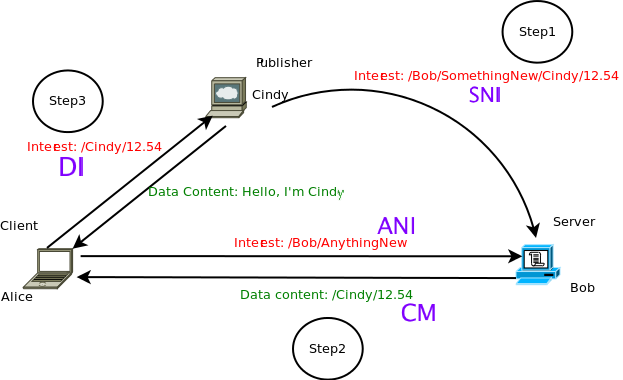
\includegraphics[width=4.5in]{png/synchronization.png}
\caption{同步消息传递过程和消息本体的获取}
\label{fig:sync_process}
\end{figure}


本章,我们将描述在系统中到底是如何同步的。
如图\ref{fig:sync_process}所示,子节点向其父节点发送SNI来通知他有一个新的消息。
控制节点然后会回复他保存的待决定的ANI,其中包含这个新的消息。
参与者通过分布式的方式获取消息实体。图\ref{fig:multi_sync}显示了多层拓扑的同步。
每个节点都会通过发送SNI和满足ANI来向上和向下传递控制信息。

\subsection{新消息通知兴趣包}
当一个节点产生一个新的消息,或者他收到来自下层节点的Something New Interest(SNI),他会将此消息向上传递给自己的控制节点。

当一个参与者产生一个新的数据,他将会做下面这些事:
\begin{enumerate}
  \item 添加这个数据进入自己本地的数据存储器
  \item 将自己的标签加入这条记录中,并且将这条记录放入自己的记录存储器。
  \item 向他的控制节点发送SNI,其中包含他的标签和实际数据的NDN名字。
  \item 处理来自子节点的待处理的ANY
\end{enumerate}

注意到SNI在其后面包含了真是的数据名字,所以当控制节点收到此SNI后,他可以立即将这个消息向上或者向下传递。

\subsection{同步兴趣包}
为了得到控制信息,每一个节点都会周期性的向他的控制节点发送带有他当前最新标签的Anything New Interest(ANI)。
当一个控制节点收到这个兴趣包时,他会将其中包含的标签信息和他自己的最新标签做对比。
有如下三种情形:
\begin{enumerate}
  \item 此标签和他自己的标签时间相同。
这时候,他将会把这个兴趣包保留为待处理的同步兴趣包,这样能够在他有状态变化时第一时间将此变化回复给其客户端。
  \item 收到的兴趣包中包含的标签晚于自己当前的标签。
这时候,他比较这个记录的时间,找到本地记录中所有比此标签新的记录,然后将所有记录返回给该兴趣包。
  \item 在自己的记录中没有此标签对应的用户信息。
这种情况下,需要将所有的记录都发送给子节点。
\end{enumerate}

当子节点收到ANI的数据包时,他会做如下的事:
\begin{enumerate}
  \item 将记录从数据中提取出来
  \item 更新自己当前的记录存储器
  \item 处理待处理的同步兴趣包
  \item 发送兴趣包以获取消息实体
\end{enumerate}

一般的,控制器控制着其内部的同步,所以其所有的子节点都会有这个控制器的标签信息。
所以大部分情况下,组内的节点只需要将他的父节点的控制信息包含在ANI中皆可以完成同步。
当这个系统处于稳定状态,所有的节点都发送相同的ANI,这些ANI是可以被NDN路由器聚合的。
而数据又是通过相反的路径精确的到达每个参与者。
当一个节点移动到另一个组内,或者控制器宕机或下线了,该节点将会找到一个新的控制器。
这种情况下,使用他先前的控制器的标签就不行了。
这种情况下,他将自己知道的所有标签发送给新的控制器。
这种模型的设计可以提供天然的对于鲁棒性和移动性的支持,我们将在第八节讨论。

\begin{figure}
\centering
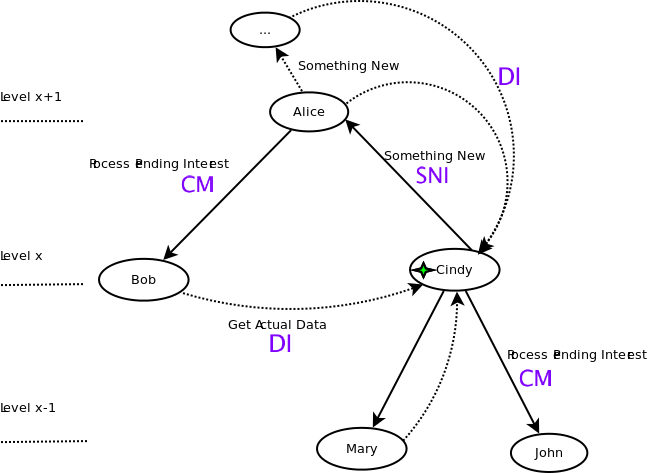
\includegraphics[width=4.5in]{png/tree-synchronization.png}
\caption{跨层的数据同步示意图}
\label{fig:multi_sync}
\end{figure}

\section{消息本体获取}

多层控制节点所同步的是控制信息,告诉每一个用户什么时候到什么地方去取数据.

节点得知正确的内容所在的地址(其名称)后,直接向这个地址发interest获取消息本体。这时候使用的是第四种Interest类型:Data Interest.

由于一个节点产生的消息的名字在NDN中是固定不变的,所有人所发送的DI都是相同的.
这样的话,所有其他节点发送的此兴趣包能够充分利用NDN的聚合效果,即NDN会将所有的重复的兴趣包过滤掉,只传输一份到下一跳路由.

同时,当有内容返回时,NDN路由还会缓存这个兴趣包,这样以后的索取此兴趣包的用户就可以在中间路由上得到满足,延迟和链路负载就会大大减少.

\section{鲁棒性和移动性支持}

\begin{figure}
\centering
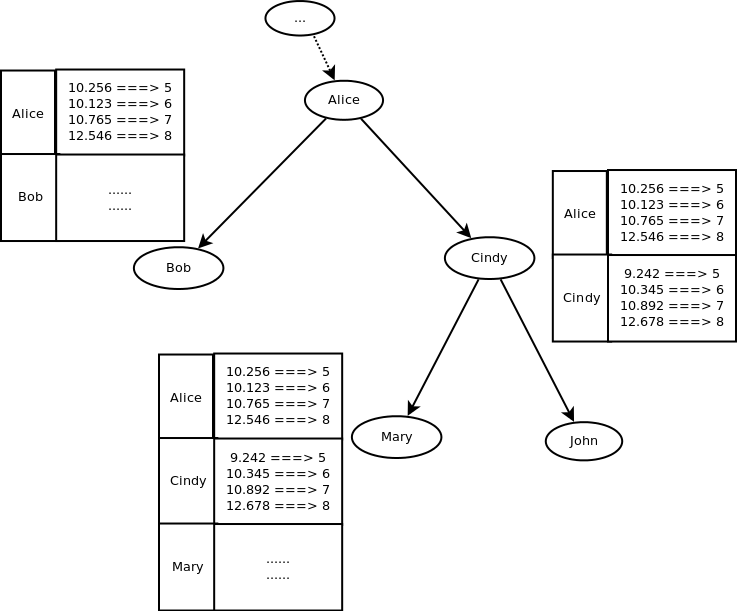
\includegraphics[width=4.5in]{png/mobility.png}
\caption{鲁棒性和移动性支持}
\label{fig:mobility}
\end{figure}

\subsection{鲁棒性}
我们的设计是一个分布式的设计,不要求有一个固定的服务器来控制整个系统的同步.
任何一个控制节点出了问题,都可以从其子节点中选出一个来替代它,具有很好的鲁棒性.

在系统稳定时,每个节点都会不停地向其父节点发送心跳包,用以确定父节点的存在性.
如果一个节点因为某种原因下线了,那么其子节点会立刻发现这一点,并且将自己的控制节点清空.
然后,这些子节点会进入控制器产生循环中,向周围广播ANI兴趣包.

按照前述算法,所有的子节点中会产生一个控制器,来代替下线的节点,并继续控制这个组的控制信息的更新与传输.

\subsection{移动性}
当一个节点移动后,其上层节点很有可能共享同一个上层节点。所以还是可以使用其时间标签正常同步。

当节点移动时,有如下三种情况:
\begin{enumerate}
  \item 该节点移动到另一个地方,但是连接到同一个控制节点.
  这种情况下,他仍然会向这个控制节点发送兴趣包以索取控制信息,不受任何影响.
  \item 该节点移动到一个较远的地方,连接到不同的控制节点.
  这个时候,他就不能使用原来的控制节点的标签进行同步了.
  然而,由于多层控制节点是和实际拓扑紧密相关的,很有可能的是,他和新的控制节点共享同一个更上层的控制器.
  这时候,他只需要把自己上层的所有节点的标签发送给新的控制器,就可以保证能继续同步.
  事实上,每个节点最终应该会共享至少顶层控制器.
  例如,在图\ref{fig:mobility}中,如果Mary移动了,并且到Bob旁边,她将连接上Bob,作为其控制节点.
  此时,Mary不能再用Cindy的标签进行同步,但是,Mary可以使用与Bob共享的Alice的标签做同步.
  因为Bob和Mary都持有Alice的标签,他们可以相互认识并继续同步.
  \item 该节点移动到一个完全陌生的环境,连顶层节点也不是共享的.
  这可能是由于暂时或永久的隔离引起的.
  考虑这种情况过于极端,因为如果顶层节点不相同,那么实际拓扑也是断的,即没有一条链路是可以让这两个群体相互通讯的.
\end{enumerate}

\section{TreeSync是如何克服ChronoSync的缺点的}

前文介绍了ChronoSync以及其缺点,在本节中,我们将讨论我们的设计是如何克服这些缺点的.

\subsection{并发消息产生}

\begin{figure}
\centering
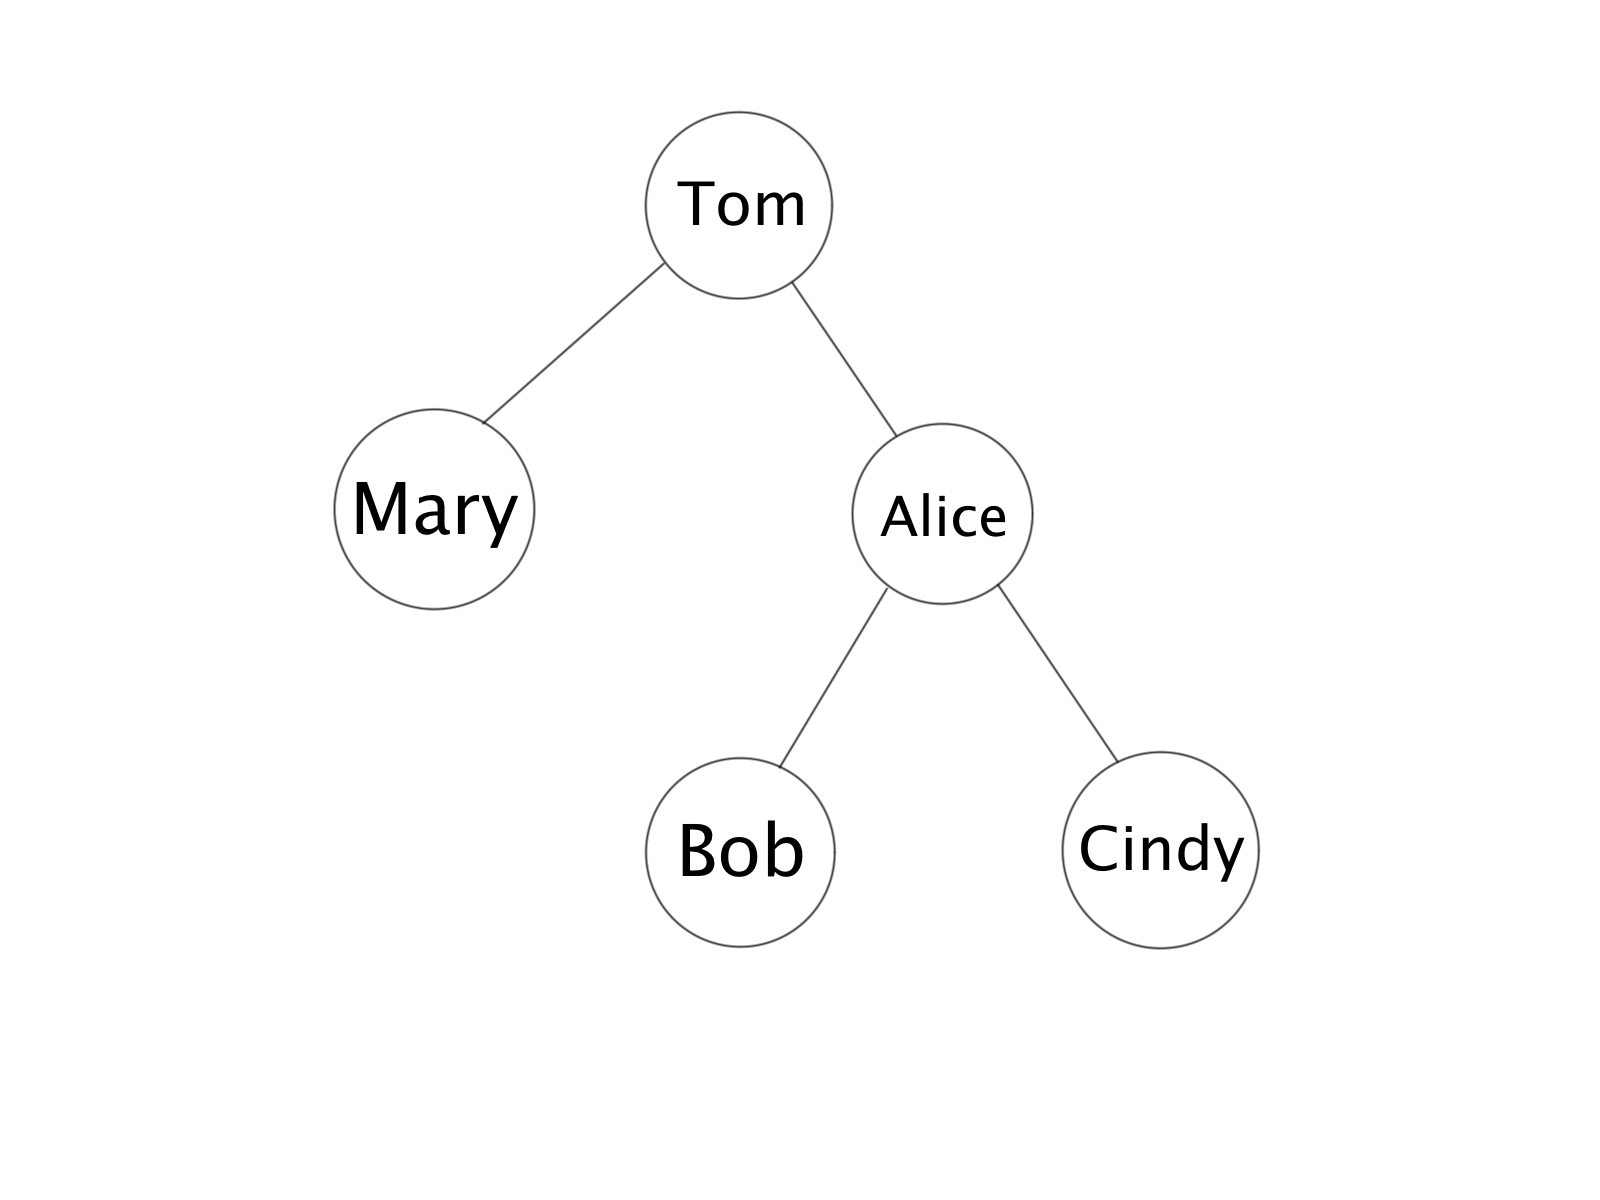
\includegraphics[width=4.5in]{png/merit.png}
\caption{处理并发消息的产生}
\label{fig:merit}
\end{figure}

TreeSync的设计使得他有很强的控制能力.
考虑图\ref{fig:merit},我们考虑如下三种情况:从上层来的两个并发消息;一个上层和一个下层消息;两个从其子节点来的下层消息.

当Tom和Mary同时产生了消息,Tom的消息会直接通过回复Alice的ANI而到达Alice.
当Mary的消息到达Tom,他将会回复Alice的另一个ANI,从而将消息转给Alice.
如果Mary的消息先到达Tom了,Tom还没来的及发送他自己的控制信息,那么他可以将这两个消息打包在一起,同时发送给Alice.

第二种情况中,如果Tom和Bob同时向群中发送消息,无论哪一个先到达Alice,都会由Alice决定消息的顺序,然后将其转发给Cindy.

第三种情况,如果Bob和Cindy同时产生消息,那么它们都会传向Alice.
Alice来对这些消息进行排序,并将控制信息向上和向下传播.

\subsection{扩展性}

ChronoSync没有层级结构,消息是直接广播给群体的,所以没有扩展性,不能用于较大的拓扑.
然而,TreeSync的设计是分层的,每一层都有控制器来掌控所有子节点的控制信息的同步.
因此,消息传递的复杂度相对于群体的人数和拓扑结构是指数下降的.
这保证了TreeSync可以用于更大的拓扑中.

  \chapter{仿真}
\label{chapter:simu}

\section{概述}

\begin{figure}
\centering
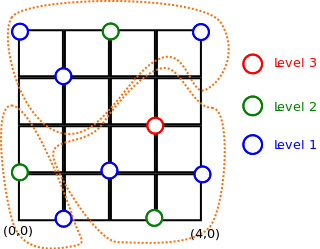
\includegraphics[width=4.5in]{png/paper-topo.png}
\caption{5x5网格型拓扑和产生的属性拓扑}
\label{fig:paper_topo}
\end{figure}

我们在ndnSIM上实现了TreeSync的仿真。
ndnSIM是Network Simulation(NS3)的一个模块,用于提供一个NDN的IP层的包装。
作为对比,我们同样实现了一个ChronoSync的ndnSIM版本。
在这一章中,我们首先验证逻辑的正确性和功能的实现。
然后我们在overhead和传输时延上做评估。

使结果更具一般性,我们采用如图\ref{fig:paper_topo}的5x5的网格拓扑结构。
网格中的每一个节点都代表一个参与者,所以总共更有25个节点。
拓扑图可能看起来很简单,但是实际上它包含6种不同环境中的节点,最大8跳的路由。
我们认为这个拓扑可以很好的代表一个一般的脱兔结构。
树形拓扑按照之前描述的算法生成。
所有的链路都具有10ms的延迟和1Mbps的带宽。
我们让参与者随机的生成新的数据,并且我们改变他们生成数据的频率来研究变化趋势。
每个人产生信息的周期是独立的。

\section{功能实现}

\begin{figure}
\centering
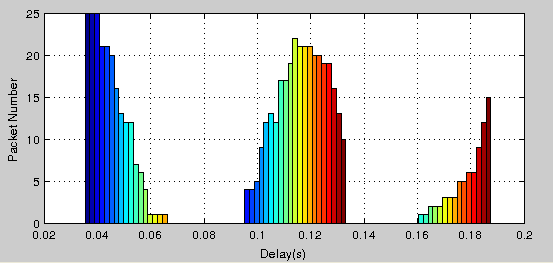
\includegraphics[width=4.5in]{png/function-delay.png}
\caption{节点收到数据的延迟}
\label{fig:function_delay}
\end{figure}

1.控制节点产生。
在网格拓扑中,控制节点产生像预期一样工作。
产生了一个四层的拓扑,最高级的控制节点在节点(3,2)上。

2.消息同步。
所有的消息都能够成功的传递给聊天室的所有人,不会丢失任何消息。
图\ref{fig:function_delay}显示了当产生频率为$2/7Hz$时的时延。从图中可以看出,时延被分为三个部分。
很快,平均,和稍慢。这是和树形拓扑紧密相关的。
如果接收者在消息产生者很近的位置,他们在树形拓扑中也会距离很近,这样他就能够很快得到控制信息,进而获取实际消息实体。
然而,当两个参与者在树形拓扑中相距很远时,控制信息要跨越好几个层级才能到达,导致了相对更大的时延。


\section{效果评估}

\subsection{链路负载}

\begin{figure}
\centering
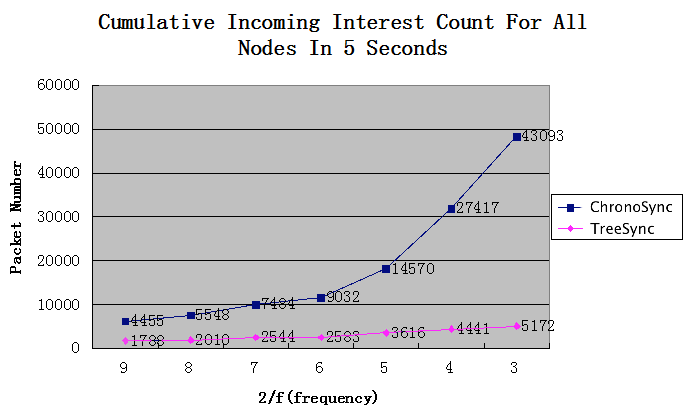
\includegraphics[width=4.5in]{png/all-incoming-interest-revised.png}
\caption{所有节点的进入的兴趣包数目}
\label{fig:overhead}
\end{figure}
\begin{figure}
\centering
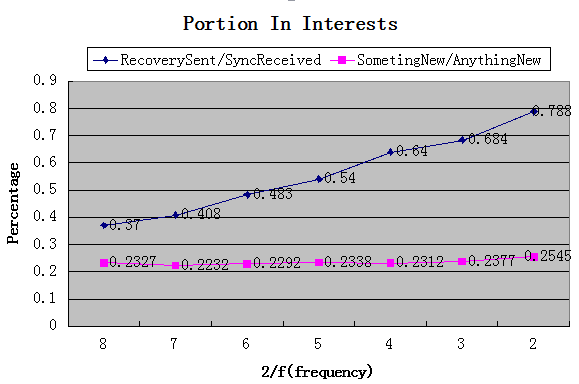
\includegraphics[width=4.5in]{png/portion-in-interests.png}
\caption{兴趣包中不同成分所占的比例}
\label{fig:interest_percentage}
\end{figure}

我们的设计在控制性上面有很大的优势,所以在overhead上会比ChronoSync有显著的减少。
在我们的试验中,我们改变消息声称的平率,然后观察overhead的变化。
在图\ref{fig:overhead}中,当频率增加时,我们的设计在包数统计上会有线性的增加,然而ChronoSync却遭受了指数的增长。
这是因为当产生消息的频率增加时,同时产生消息的频率也指数增加,那么ChronoSync就必须发送额外的恢复兴趣包来处理这种冲突。
注意到我们使用的是所有进入的兴趣包的数目统计,因为它可以代表整个状态。
NDN路由器的聚合性也可以减少进入的兴趣包数。
从图\ref{fig:interest_percentage}可以看出,
在ChronoSync中节点需要发送恢复兴趣包的比例随着频率增长得非常快,
然而在我们的设计中,SNI和ANI的比例基本保持不变。

\subsection{延迟}

\begin{figure}
\centering
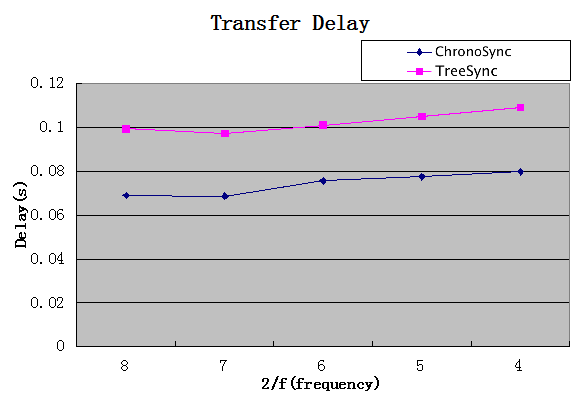
\includegraphics[width=4.5in]{png/delay-compare-revised.png}
\caption{延迟比较}
\label{fig:delay_compare}
\end{figure}

\begin{figure}
\centering
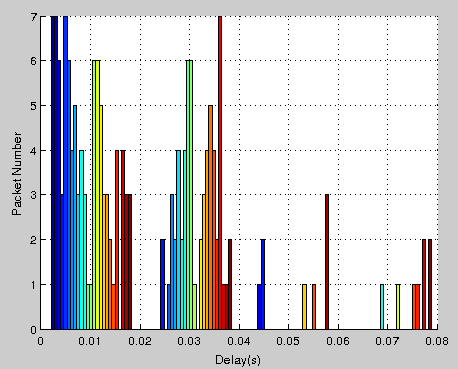
\includegraphics[width=4.5in]{png/data-fetch-delay.png}
\caption{数据获取兴趣包拉回数据的延迟}
\label{fig:data_fetch_delay}
\end{figure}

由于控制信息要经过多层控制器,即时拓扑结构和实际拓扑是紧密相关的,延迟效果依然比完全按照最有路径的ChronoSync稍差。
但是,当数据产生更加频繁时,ChronoSync需要发送更多的恢复兴趣包,并且当带宽不足时会增加其时延。
如图\ref{fig:delay_compare}所示,TreeSync的时延要稍大于ChronoSync,但是仍然很好,并且两种方法都大幅度优于IP网络模型解决方案。
考虑到获得的巨大的控制性能,这种权衡牺牲是值得的。

另一点,在我们的数据中,实际数据的获取是完全分布式的,可以充分利用NDN结构的优点。
图\ref{fig:data_fetch_delay}显示了参与者从发送实际消息请求到得到数据的延迟,可以看到这个过程非常迅速。
并且这种设计也为低时延和小overhead做出了贡献。

  \chapter{总结}
\label{chapter:conclude}

\section{项目完成情况}

在这篇论文中,我们提出了基于NDN网络的解决即时多人聊天应用的新的算法,TreeSync。
TreeSync充分利用了传统中央服务器式模型和NDN的有效的分布式特性。

首先,多层控制节点可以提供强大的控制能力,来处理复杂的情形。
其次,该设计的本质的分布式特征让它能够有效率的获取消息,并且具有鲁棒性和移动性支持,享有极小的overhead。
另外,树形结构的层级设计也为扩展性提供了保证。当节点增多时,复杂度是指数下降的。

我们在ndnSIM上实现了TreeSync,并且评估了其性能。消息能够正确而快速的在群体中相互同步。
在拥有较快同步时延的同时,overhead相对于其他算法有显著的降低。

\section{目前存在的问题}

目前,当拓扑结构较大时,仍然存在问题,延迟较大.
导致问题的关键因素是,当控制节点满足子节点的同步兴趣包后,该数据包必须到达子节点,
然后子节点才能发送新的同步兴趣包来获取接下来的同步消息.
这同时也是NDN的客户端主导数据传递的模型所具有的弊端:数据无法直接发送,必须通过兴趣包拉回.

解决此问题需要NDN的内部路由机制的改变:
NDN中应该存在一种Interest,其索取的不是单一数据,而是一个数据流.
当有数据要返回时,该Interest不会失效,而是继续存在,以获取接下来的消息.
这也是我们实验室的一个研究方向.

\section{未来的展望}

消息同步问题在NDN中解决,可以充分利用NDN的分布式特性,使得性能比现有网络的解决方案有明显的优势.
未来随着NDN的更加成熟和更大范围的部署,NDN中得应用将会得到更好地发展.

未来的研究方向主要有如下几点:
优化拓扑生成过程,使生成的树形拓扑更加合理和高效;
基于流的Interest用于消息同步系统;
使用NDN的Javascript库开发跨平台的更高性能的群聊应用Demo.


%%%%%%%%%%%%%%%%%%%%%%%%%%%%%%
%% 附件部分
%%%%%%%%%%%%%%%%%%%%%%%%%%%%%%
\backmatter

  % 参考文献
  % 使用 BibTeX
  % 选择参考文献的排版格式。注意ustcbib这个格式不保证完全符合要求,请自行决定是否使用
  \bibliographystyle{ustcbib}%{GBT7714-2005NLang-UTF8}
  \bibliography{bib/tex}
  \nocite{*} % for every item
  % 不使用 BibTeX
  % %\renewcommand{\baselinestretch}{0.5}
\begin{thebibliography}{10}

\bibitem{deng:01a}
{邓建松,~彭冉冉,~陈长松邓建松,~彭冉冉,~陈长松邓建松,~彭冉冉,~陈长松邓建松,~彭冉冉,~陈长松邓建松,~彭冉冉,~陈长松邓建松,~彭冉冉,~陈长松邓建松,~彭冉冉,~陈长松邓建松,~彭冉冉,~陈长松邓建松,~彭冉冉,~陈长松邓建松,~彭冉冉,~陈长松邓建松,~彭冉冉,~陈长松}.
\newblock {\em \LaTeXe{}~科技排版指南}.
\newblock 科学出版社,~书号:~7-03-009239-2/TP.1516, 北京, 2001.

\bibitem{wang:00a}
王磊.
\newblock {\em \LaTeXe{}~插图指南}.
\newblock 2000.

\bibitem{zhang:03a}
张林波.
\newblock {\em 关于新版~CCT~的说明}.
\newblock 2003.

\bibitem{lshort-cn}
C\TeX{} 翻译小组.
\newblock {\em lshort~中文版~3.20}.
\newblock 2003.

\bibitem{knuth86e}
Donald~E. Knuth.
\newblock {\em Computer Modern Typefaces}, volume~E of {\em Computers and
  Typesetting}.
\newblock Addison-Wesley, Reading, Massachusetts, 1986.

\bibitem{knuth86d}
Donald~E. Knuth.
\newblock {\em {METAFONT}: The Program}, volume~D of {\em Computers and
  Typesetting}.
\newblock Addison-Wesley, Reading, Massachusetts, 1986.

\bibitem{knuth86c}
Donald~E. Knuth.
\newblock {\em The {METAFONT}book}, volume~C of {\em Computers and
  Typesetting}.
\newblock Addison-Wesley, Reading, Massachusetts, 1986.

\bibitem{knuth86b}
Donald~E. Knuth.
\newblock {\em {TeX}: The Program}, volume~B of {\em Computers and
  Typesetting}.
\newblock Addison-Wesley, Reading, Massachusetts, 1986.

\bibitem{knuth86a}
Donald~E. Knuth.
\newblock {\em The {TeX}book}, volume~A of {\em Computers and Typesetting}.
\newblock Addison-Wesley, Reading, Massachusetts, 1986.

\bibitem{lamport85a}
Leslie Lamport.
\newblock {\em {LaTeX} --- A Document Preparation System: User's Guide and
  Reference Manual}.
\newblock Addison-Wesley, Reading, Massachusetts, 2nd edition, 1985.

\end{thebibliography}


  % 附录,没有请注释掉
  % \begin{appendix}
  %   \include{chapter/chap-req}
  % \end{appendix}

  \makeatletter
  \ifustc@bachelor\relax\else
    % 致谢
	
\begin{thanks}


在中国科技大学完成本科学业的四年里,我所从事的学习和研究工作,都是在导师以及系里其他老师和同学的指导和帮助下进行的。
在完成论文之际,请容许我对他们表达诚挚的谢意。

首先感谢导师谭小彬副教授这一年的指导和教诲,是他们把我带到了未来网络的研究领域。
在完成毕业设计的过程中,每一次与谭老师的讨论都让我的思路更清晰,他的一针见血的提问不断纠正我前进的方向.
谭老师严谨的研究态度及忘我的工作精神,认真细致的治学态度及宽广的胸怀,都将使我受益终身。

感谢班主任陈金雯老师多年的关怀。
感谢朱明,郑烇等老师,他们的指导给我本科阶段的研究工作打下了基础。

感谢周子健、周自飞、武帆等师兄师姐们的指点和照顾;
感谢肖琪、赵志凡、陈杨斌等几位同班同学,与你们的讨论使我受益良多;
我们在1316实验室共同学习共同生活,一起走过了这段愉快而难忘的岁月。

感谢科大,感谢一路走过来的兄弟姐妹们,在最宝贵年华里,是你们伴随着我的成长。

最后,感谢我家人一贯的鼓励和支持,你们是我追求学业的坚强后盾。

\vskip 18pt

\begin{flushright}

~~~~李合璧~~~~

\today

\end{flushright}

\end{thanks}
%硕博致谢部分
    % 发表文章目录
    
\chapter{在读期间发表的学术论文与取得的研究成果}

\noindent\textbf{研究工作:}

\begin{enumerate}

\item A A A A A A A A A
\item A A A A A A A A A
\item A A A A A A A A A
\item A A A A A A A A A

\end{enumerate}


\noindent\textbf{已发表论文:}

\begin{enumerate}

\item A A A A A A A A A 
\item A A A A A A A A A
\item A A A A A A A A A
\item A A A A A A A A A
\item A A A A A A A A A
\item A A A A A A A A A
\item A A A A A A A A A
\item A A A A A A A A A

\end{enumerate}

\vskip 1cm

\noindent\textbf{待发表论文:}

\begin{enumerate}

\item A A A A A A A A A

\end{enumerate} 
  \fi
  \makeatother

\end{document}
